\chapter{Introduction}
\label{intro}

\section{The Standard Model}
The Standard Model of particle physics (SM) describes all known particles and their non-gravitational interactions. Developed and experimentally verified over the past six decades, the SM posits the existence of twelve spin-$\frac{1}{2}$ particles, the fermions, that make up all observed matter; twelve spin-1 particles, the gauge bosons, that communicate the electromagnetic, weak, and strong forces; and one fundamental scalar, the Higgs boson, which breaks electroweak symmetry, giving mass to the gauge bosons and fermions.

The fermions and gauge bosons can be classified according to the forces with which they interact. The fermions are further divided into six quarks, which carry color and interact via the strong force, and six leptons, which do not. Furthermore, all six quarks and three of the leptons (the electron, muon, and tau) carry electric charge and interact electromagnetically. All fermions interact via the weak force. The gauge bosons include the photon, which communicates the electromagnetic force; the $\mathrm{W}^+$, $\mathrm{W}^-$, and $\mathrm{Z^0}$, which communicate the weak force; and eight gluons that communicate the strong force. Of these, only the $\mathrm{W}^+$ and $\mathrm{W}^-$ are electrically charged and only the gluons carry color charge. Finally, the fermions are grouped into three generations, each with two quarks, one charged leptons, and one neutral lepton.  Figure~\ref{sm_particles} shows how the SM particles are organized and lists some of their properties.
\fxnote{cite something}
\fxnote{what about flavor? what about saying the word neutrino?}

\begin{figure}
\centering
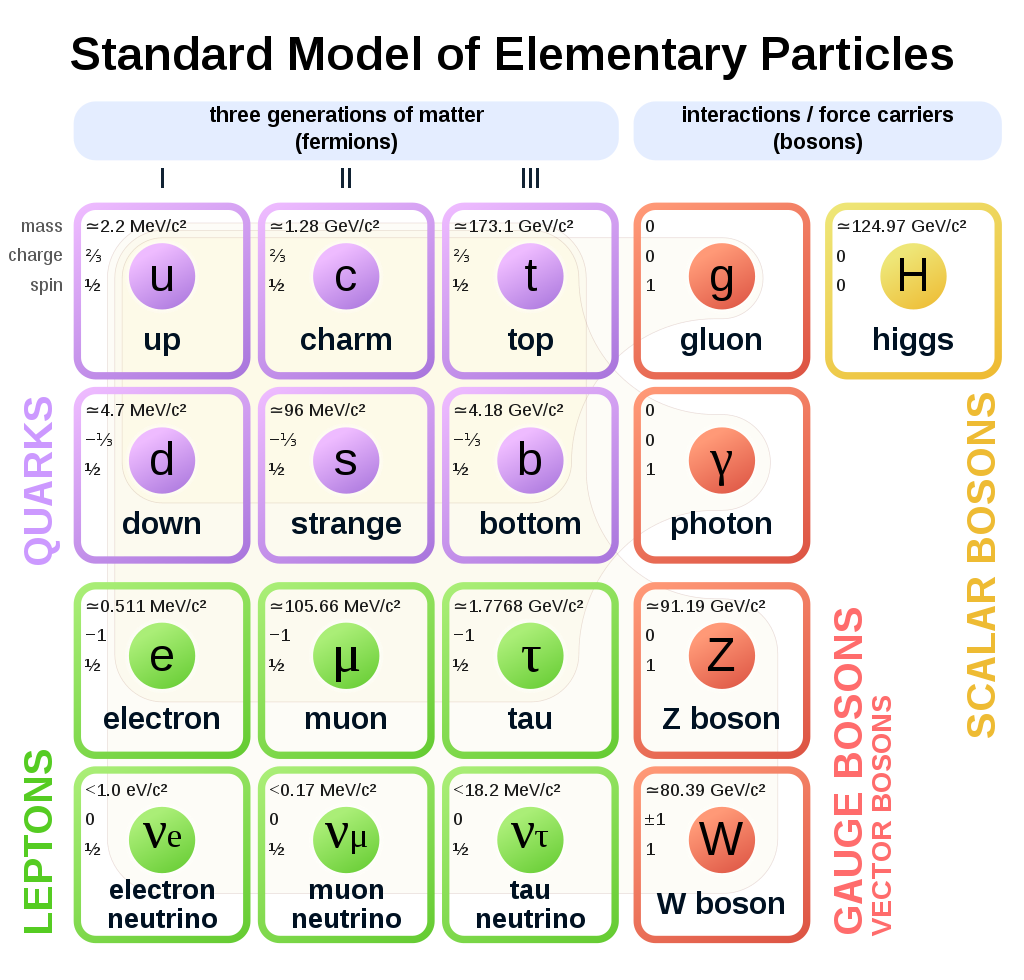
\includegraphics[scale=0.4]{figures/intro/sm_particles.png}
\caption{The Standard Model particle content.}
\label{sm_particles}
\end{figure}

In the SM, the interactions between particles are governed by two theories: quantum chromodynamics (QCD), which describes the strong force, and the electroweak theory, which describes the electromagnetic and weak forces. The following sections will provide a brief overview of these theories.

\subsection{Quantum chromodynamics}
QCD describes the strong interactions between quarks and gluons and is based on the $SU(3)_{c}$ symmetry group, where the subscript c refers to color charge. In QCD, all quarks and gluons carry color charge, which allows interactions between two quarks and a gluon, three gluons, or four gluons. QCD is responsible for the formation of all hadrons (such as protons and neutrons), and leads to two unique phenomena: confinement and asymptotic freedom. \fxnote{quarks transform as triplets, 3 color charges, developed in the 70s, ?}

Confinement refers to the experimental fact that an isolated particle with color charge has never been directly observed. Composite particles composed of quarks and gluons are always neutral under color, and attempts to separate the constituent particles will only produce new hadrons. This phenomenon is the result of the unique running of the strong coupling constant, which increases with decreasing energy (and therefore increasing distance). \fxnote{energy, momentum transfer, interaction energy?} \fxnote{mention dis?} \fxnote{mention jets?}

Asymptotic freedom shows up at the opposite end of the energy spectrum. In high energy interactions (such as those at the Large Hadron Collider), the strong coupling constant is small enough to render the quarks nearly free. In this regime, the small coupling constant enables perturbative calculations. \fxnote{say why this matters, especially if it matters for lhc stuff}

\subsection{The electroweak theory}
The electroweak theory unifies the electromagnetic and weak interactions and is based on the $SU(2)_{L} \otimes U(1)_{Y}$ symmetry group. The electroweak theory posits two new charges: weak isospin, which has three components $T_{1,2,3}$, and hypercharge, $Y$. $T_{3}$ is $\pm\frac{1}{2}$ for all left-handed fermions and 0 otherwise, while Y varies according to $Q=T_{3}+\frac{1}{2}Y$, where $Q$ is the familiar electric charge. Each generation of left-handed quarks or leptons forms an SU(2) doublet. The first generation doublets, for example, are:
\begin{equation}
    \binom{\nu_{e}}{e^{-}}_{L},\ \binom{u}{d}_{L}
\end{equation}
where, as in $SU(2)_{L}$, the L denotes left-handed chiral states. The three generators of $SU(2)_{L}$ result in three massless spin-1 bosons: $W1$, $W2$, and $W3$, while $U(1)_{Y}$ gives rise to one massless spin-1 boson, $B^{0}$. When all is said and done, the physical $W^{\pm}$ bosons are identified as superpositions of $W^{1}$ and $W^{2}$ while $Z^0$ and the photon are identified as superpositions of $W^{3}$ and $B^{0}$.
\fxnote{cp violation, mixing between generations, right-handed neutrinos, mass terms not allowed?}

\subsection{The Higgs mechanism}

\subsection{Current status}





% higgs mechanism
% what's missing
% hierarchy problem
\section{Beyond the Standard Model}
% overview
% susy as a solution to hierarchy problem
% general motivation to look for llps
% displaced susy
